\subsection{Analog-to-Digital Converter} \label{sec:ADC_imp}
Mikrokontrolleren, der avendes som løsningsstrategi i \autoref{sec:loesningsstrategi}, har en Sucessive Approximation Register (SAR) ADC, som gør det muligt at konvertere det analoge signal til et digitalt. 
Der ønskes en konfigurering af tre analoge kanaler, herunder Y-aksen på begge accelerometre samt output fra EMG-forstærkeren. 
Opsætningen af ADC'en på mikrokontrolleren fremgår af \autoref{fig:ADC_teori}, hvor en yderligere beskrivelse kan læses af \autoref{sec:ADC_bilag}.

\begin{figure}[H]
\centering
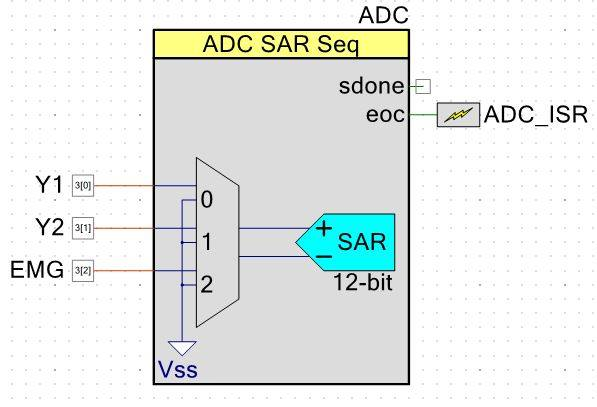
\includegraphics[width=0.5\textwidth]{figures/implementering/ADC_imp.jpg}
\caption{ADC'ens opsætning på PSoC. SAR er ADC-typen. Kanalerne Y1, Y2 og EMG modtager signaler fra henholdsvis accelerometret, der er placeret parallelt med femur, accelerometret, der er placeret parallelt med tibia, og EMG-signal. sdone er en outputterminal, der signalerer, at ADC'en har samplet det aktuelle input. End of conversion (eoc) signalerer, når en konversionscyklus er gennemført, dermed kan værdierne fra de samplede kanaler aflæses i samplingsregistret. Når eoc signalerer dette laver ADC'ens Interrupt Service Routine (ISR), som fremgår som ADC\_ISR, et interrupt, hvor værdierne for samplingsregisterer aflæses \citep{ADC2014}.}
\label{fig:ADC_teori}
\end{figure}

\noindent
Da ingen af input-signalerne er differentielle, opsættes ADC'en til at måle single ended. Hvert negativt input for kanalerne er derfor tilkoblet $V_{ss}$, der fungerer som jord. 
Der vælges en 12 bits-konfiguration af ADC'en, da dette er den højest mulige bit-værdi.
Da der anvendes en single ended konfiguration af kanalerne, svarer dette til, at ADC'en anvender 11 bit. 
ADC'ens arbejdsområde er defineret til $3,3~V$, hvoraf LSB'en for ADC'en kan beregnes ud fra \autoref{equ:LSB}, hvilket giver $1,61~mV$. 
Hvis der sker ændringer i signalet, der er mindre end LSB på $1,61~mV$, vil dette ikke komme til udtryk i det konverterede signal. 

I ADC'en opsættes en clockfrekvens. 
Det er muligt at reducere konverteringstiden ved at øge ADC'ens clock frekvens, der kan indstilles mellem $1000~MHz$ og $9000~MHz$ \citep{ADC2014}. 
Opsætningen for ADC'en fremgår i \autoref{sec:ADC_bilag}. 
Clock cycles betegner tiden mellem to efterfølgende impulser fra en oscillator, og samplingtiden måles i clock cycles. 
Der er forskellige parametre, der kan indstilles i ADC'en; opløsning, samplingsrate og clockfrekvens. 
Disse parametre bestemmer ADC'ens konverteringsrate. %Konvertingstiden er den inverse af konverteringsraten. 

Da der ønskes at sample med 10 gange signalets frekvensområde, hvilket ifølge \autoref{sec:pilotforsoeg} er mellem 0,4 og $10~Hz$, vælges der at sample med $100~Hz$. 
Idet der defineres en samplingsfrekvens på $100~Hz$, oplyser ADC'en en reel samplingsfrekvens per kanal og reel clockfrekvens. 
Den reelle samplefrekvens opgives til $97~Hz$. Til at opnå den ønskede frekvens ændres i clock cycles, som beskrevet i \autoref{sec:ADC_bilag}.
Heraf opnås en konverteringstid på $3,32~ms$ for hver af kanalerne, således den reelle samplingsfrekvens opgives til $100~Hz$ og en clockfrekvens på $1600~kHz$. 

Derudover fremgår det af \autoref{fig:ADC_teori}, at outputtet fra ADC'en er tilkoblet via eoc til ADC\_ ISR. Dette er designet således, at systemet er i sleepmode mellem hvert interrupt. Idet der gives et interrupt, er data klar til at blive aflæst og behandlet fra samplingsregisteret \citep{ADC2014}.


